\documentclass{article}
\usepackage[utf8]{inputenc}
\usepackage{amsmath}
\usepackage{amsfonts}
\usepackage{amssymb}
\usepackage{graphicx}
\usepackage{geometry}
\usepackage{xcolor}
\usepackage{gensymb}
\usepackage{hyperref}
\usepackage{gensymb}
\usepackage{listings}

\newcommand{\inv}{^{-1}}   
\newcommand{\Z}{\mathbb Z}
\newcommand{\R}{\mathbb R}
\newcommand{\Q}{\mathbb Q}
\newcommand{\C}{\mathbb C}
\newcommand{\N}{\mathbb N}

\begin{document}
\pagecolor{black}
\color{white}

\medskip\noindent\textbf{1.} \begin{center}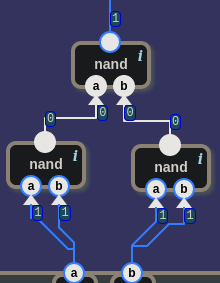
\includegraphics{or_gate.png}\end{center}    

\medskip\noindent\textbf{2.} \begin{center}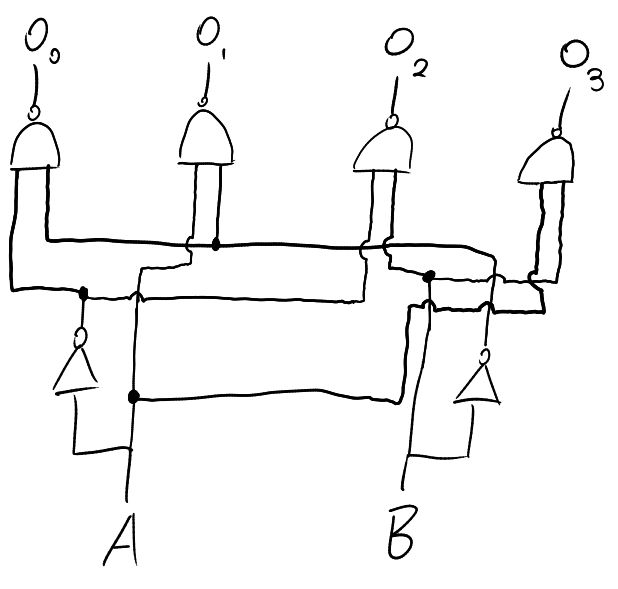
\includegraphics[scale=.5]{2-4-line.png}\end{center}

\medskip\noindent\textbf{3.}

    When the input changes from 0 to 1, the upper input to the AND gate immediately transitions from 0 to 1, but the lower input takes a few nanoseconds before it transitions from 1 to 0. Thus, there is a short period of time in which both inputs to the AND gate are 1, so the output of the AND gate is 1.

\newpage\noindent\textbf{4.}

    When the input changes from 1 to 0, the upper input to the AND gate immediately transitions from 1 to 0, but the lower input takes a few nanoseconds before it transitions from 0 to 1. Thus, there is a short period of time in which both inputs to the AND gate are 0, but there is no state in which both inputs to the AND gate are 1, so the output of the AND gate is never 1.

\medskip\noindent\textbf{5.}

    The given circuit produces a pulse on the 0-1 transition and the 1-0 transition. This is because the XOR gate's output will be high whenever its inputs are not equal, and the inputs will be different in both transition states.

\medskip\noindent\textbf{6.}

\begin{center} 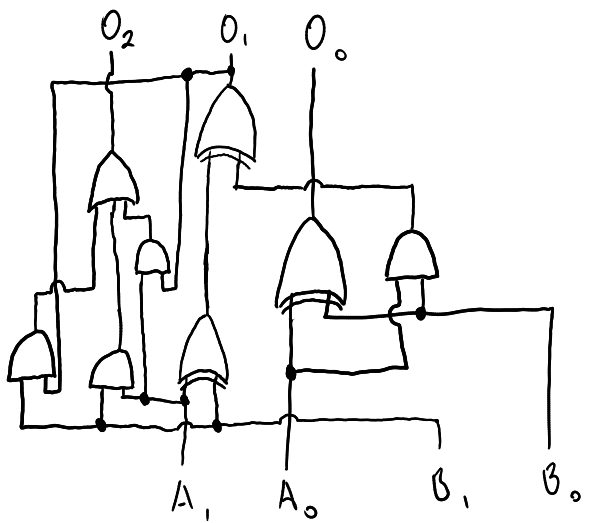
\includegraphics{6.png} \end{center}

\newpage\noindent\textbf{7.} 
    
    The following table shows the multiplication of $AB$ by $CD$, producing $EFGH$:

    \begin{center}\begin{tabular}{| c | c | c | c | c | c | c | c |}
        \hline
        $A$ & $B$ & $C$ & $D$ & $E$ & $F$ & $G$ & $H$ \\
        \hline
        0 & 0 & 0 & 0 & 0 & 0 & 0 & 0 \\
        0 & 0 & 0 & 1 & 0 & 0 & 0 & 0 \\
        0 & 0 & 1 & 0 & 0 & 0 & 0 & 0 \\
        0 & 0 & 1 & 1 & 0 & 0 & 0 & 0 \\
        0 & 1 & 0 & 0 & 0 & 0 & 0 & 0 \\
        0 & 1 & 0 & 1 & 0 & 0 & 0 & 1 \\
        0 & 1 & 1 & 0 & 0 & 0 & 1 & 0 \\
        0 & 1 & 1 & 1 & 0 & 0 & 1 & 1 \\
        1 & 0 & 0 & 0 & 0 & 0 & 0 & 0 \\
        1 & 0 & 0 & 1 & 0 & 0 & 1 & 0 \\
        1 & 0 & 1 & 0 & 0 & 1 & 0 & 0 \\
        1 & 0 & 1 & 1 & 0 & 1 & 1 & 0 \\
        1 & 1 & 0 & 0 & 0 & 0 & 0 & 0 \\
        1 & 1 & 0 & 1 & 0 & 0 & 1 & 1 \\
        1 & 1 & 1 & 0 & 0 & 1 & 1 & 0 \\
        1 & 1 & 1 & 1 & 1 & 0 & 0 & 1 \\
        \hline
    \end{tabular}\end{center}

\medskip\noindent\textbf{8.}
\begin{align*}
    E &= A \text{ AND } B \text{ AND } C \text{ AND } D \\
    F &= A \text{ AND } C \text{ AND } (B \text{ NAND } D) \\
    G &= (A \text{ AND } C) \text{ XOR } (B \text{ AND } D) \\
    H &= B \text{ AND } D
\end{align*}

\newpage\noindent\textbf{9.}

    \begin{center}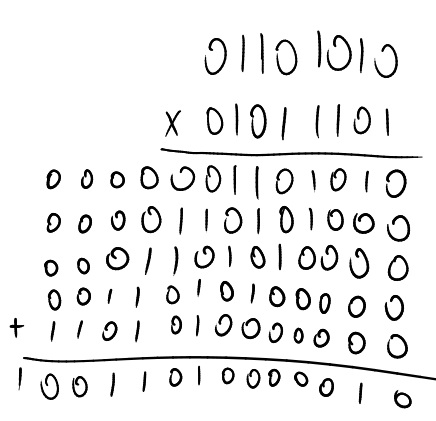
\includegraphics[scale=.5]{multiplication.png}\end{center}

    0b10011010000010 = 0x2682 = 9858

\medskip\noindent\textbf{10.}

    

\end{document}
